\documentclass{beamer}
%\usetheme{Madrid}
%\usetheme{Boadilla}
%\usetheme{default}
%\usetheme{Warsaw}
%\usetheme{Bergen}
%\usetheme{Frankfurt}
\usetheme{Darmstadt}

%\usecolortheme{seahorse}
%\usecolortheme{beaver}
\usecolortheme[named=orange]{structure}

\setbeamertemplate{footline}[page number]
%\setbeamercovered{transparent}
\setbeamercovered{invisible}
\setbeamertemplate{navigation symbols}{}

\usepackage{multimedia}
\usepackage{graphicx}
\usepackage[utf8]{inputenc}
%\usepackage[T1]{fontenc}
\usepackage[frenchb]{babel} 
\usepackage[all]{xy}
\usepackage{multirow}
\usepackage{lmodern}
\usepackage{subfigure}
\usepackage{ulem}
\usepackage{hyperref}

%% --------------

\title[Replanification rapide]{Replanification en temps réel pour\\ les robots humanoïdes}
\author{L\'eo B\textsc{audouin}}
\institute[LAAS-CNRS]
{
Stage de Master Recherche 2011\\
\medskip
{\emph{leo.baudouin@ifma.fr}}
}
\date{30 août 2011}

%% --------------

\begin{document}

\begin{frame}
\titlepage
\end{frame}

\begin{frame}
\tableofcontents
\end{frame}

%% --------------

%% \section*{Introduction}
%% \subsection*{Replanification}

%% \begin{frame}
%%   \center Replanification en robotique humanoïde
%%   \begin{figure}
%%     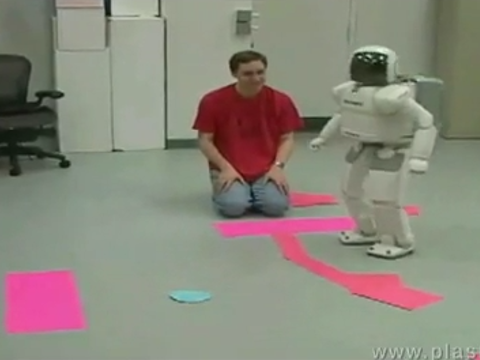
\includegraphics[width=5cm]{./images/Asimo.png}~
%%     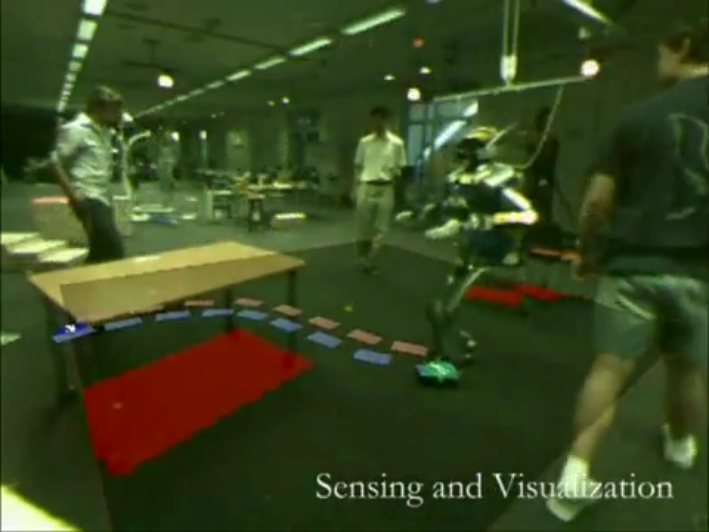
\includegraphics[width=5cm]{./images/Hrp2.png}
%%   \end{figure}
%% \end{frame}


%% \subsection*{Algorithmes existants}
%% \begin{frame}
%%   \begin{center}
%%     \movie{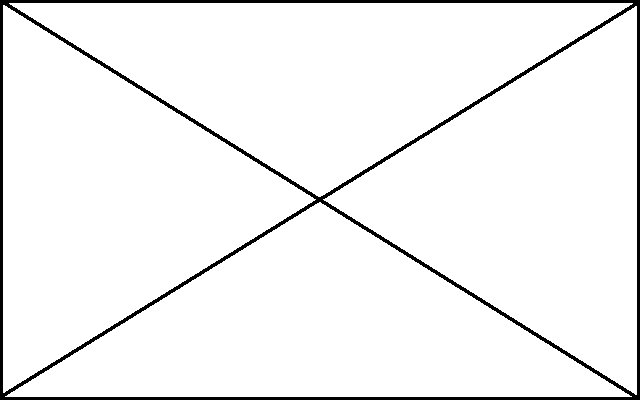
\includegraphics[width=7cm]{./images/vide.jpg}}{./videos/SteppingOverObstaclesFastPlanning.avi}\\
%%     Planification en environnement contraint.
%%   \end{center}
%% \end{frame}

% --------------

\section{Etat de l'art}
\subsection*{Littérature scientifique}
\begin{frame}
  \center Replanification en robotique humanoïde
  \begin{figure}
    \subfigure[A\textsc{simo} naviguant dans un environnement 2D mobile.]{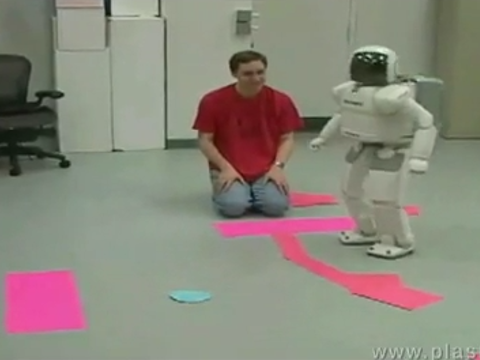
\includegraphics[width=6cm]{./images/Asimo.png}}~
    \subfigure[Pas admissibles pour la planification.]{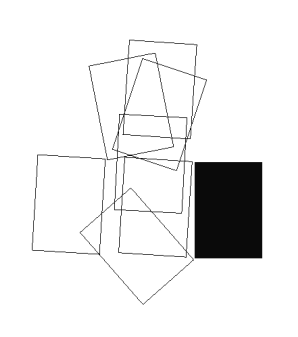
\includegraphics[width=4cm]{./images/FewSteps.png}}\\
  \end{figure}

  \begin{small}
    \emph{Footstep planning for the Honda ASIMO Humanoid}.\\
    J. Chestnutt, M. Lau, G. Cheung, J. Kuffner, J. Hodgins, and T. Kanade.\\
    \textit{In IEEE/RAS Int.Conf. on Robotics and Automation}, 2005
  \end{small}

\end{frame}

\begin{frame}
 \center Replanification en robotique humanoïde
  \begin{figure}
    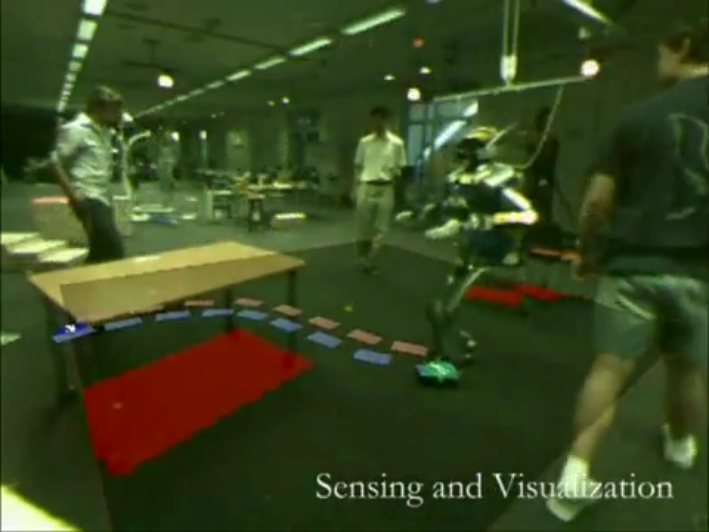
\includegraphics[width=6cm]{./images/Hrp2.png}\\
    Projections en rouge des obstacles 3D.
  \end{figure}

  \begin{small}
    \emph{Motion Planning for Humanoid Robots}.\\
    Chestnutt, K. Harada, E. Yoshida, and Y. Kazuhito.\\
    Chapter Navigation and gait planning, pages 1-28. Springer-Verlag, 2010.
  \end{small}

\end{frame}

\begin{frame}
  \begin{center}
    Planification dans un environnement contraint.\\
    \vspace{3mm}
    \movie{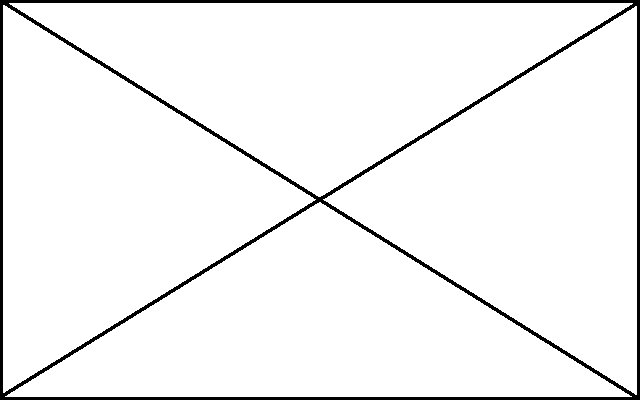
\includegraphics[width=7cm]{./images/vide.jpg}}{./videos/SteppingOverObstaclesFastPlanning.avi}\\
  \end{center}

  \begin{center}
    \begin{small}
      \emph{Fast humanoid robot collision-free footstep planning using\\ swept volume approximations}.\\
      N. Perrin, O. Stasse, L. Baudouin, F. Lamiraux, and E. Yoshida.\\
      \textit{IEEE Transactions on Robotics}, 2011.
    \end{small}
  \end{center}
\end{frame}

\subsection*{Demi-pas}
\begin{frame}
  \begin{center}
    Notion de séquence de demi-pas quasi-statiques.
    \begin{figure}
      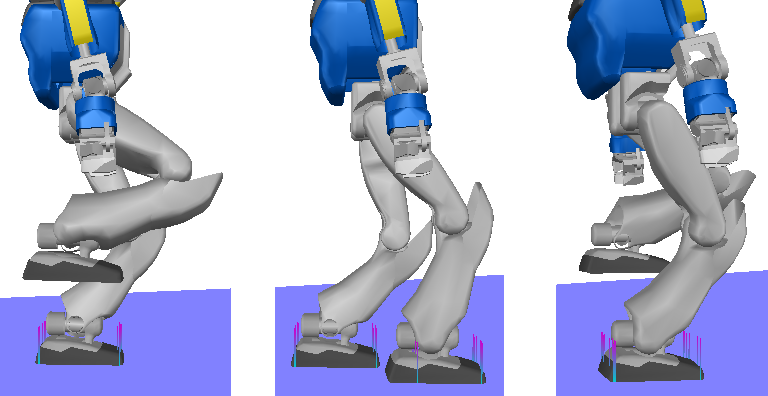
\includegraphics[width=8cm]{./images/HalfStep.png}\\
    \end{figure}
   \end{center}
  Un pas complet se fait en 4 phases :
  \begin{small}
    \begin{itemize}
    \item Phase stable de simple support
    \item Phase de vol
    \item Phase stable de double support
    \item Phase de vol
    %\item Phase stable de simple support
    \end{itemize}
    \end{small}
\end{frame}

\subsection*{RRT}
\begin{frame}
Explication du RRT
\end{frame}

% --------------

\section{Planification}
\subsection{Rapidly-exploring Random Trees - RRT}
\begin{frame}
  \center Recherche de chemin : Rapidly-exploring Random Trees (RRT)
  \begin{figure}
    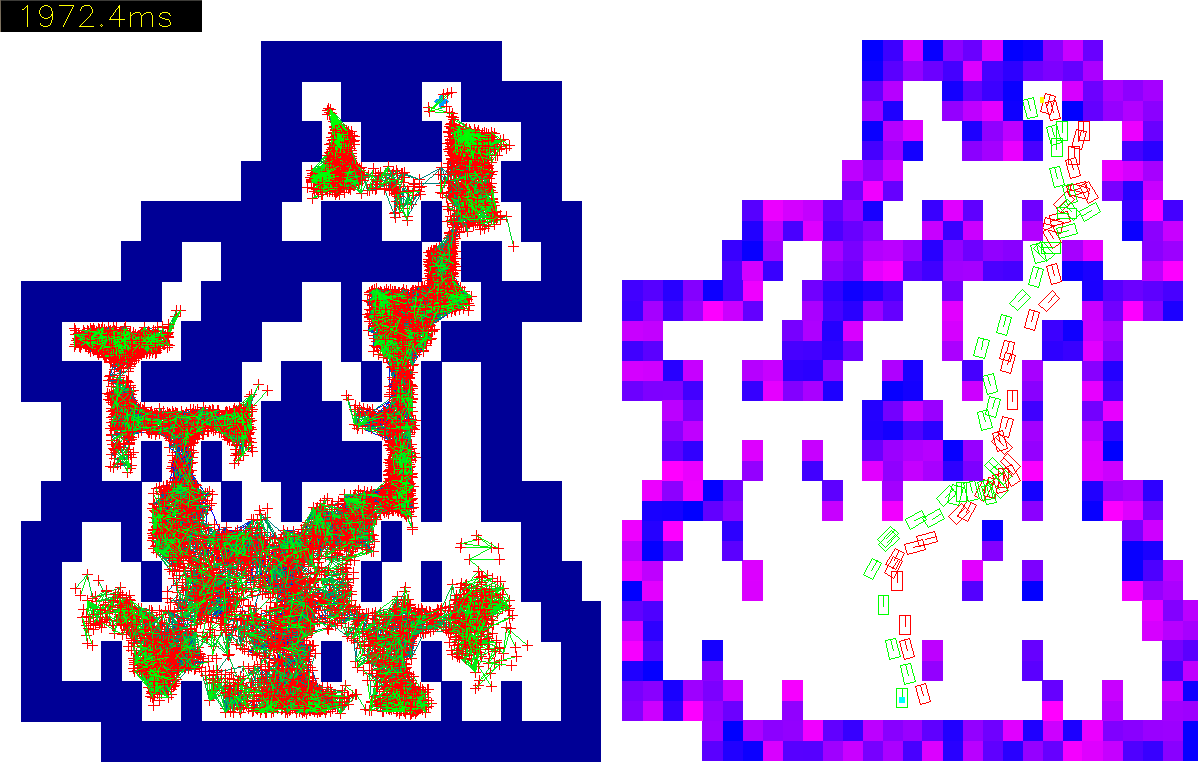
\includegraphics[width=11cm]{./images/RRT.png}
  \end{figure}
\end{frame}

\begin{frame}
  \begin{columns}
    \begin{column}{7cm}
      %\begin{columns}{1cm}
      \begin{itemize}
      \item Avantages :
        \begin{itemize}
        \item Rapidité des itérations
        \item Couverture de l'espace
        \item Evite les miminums locaux
        \item Nombre de pas admissibles important
        \end{itemize}
        \vspace{3mm}
      \item Inconvénients :
        \begin{itemize}
        \item Trajectoires non-optimales
        \item Imprévisible
        \end{itemize}
      \end{itemize}
    \end{column}

    \begin{column}{4cm}
      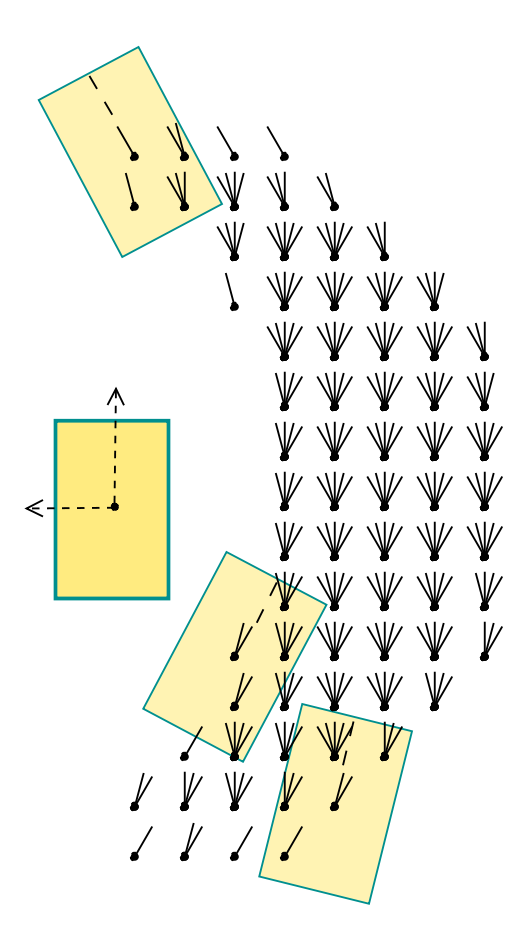
\includegraphics[width=3cm]{./images/grid_simple.png}
    \end{column}
  \end{columns}

  \vspace{5mm}
  Exemple : Vitesse de création d'un arbre RRT avec des obstacles.
\end{frame}


\subsection{Proximity Query Package - PQP}

\begin{frame}
  \begin{center}
    Détection de collision
    \begin{figure}
      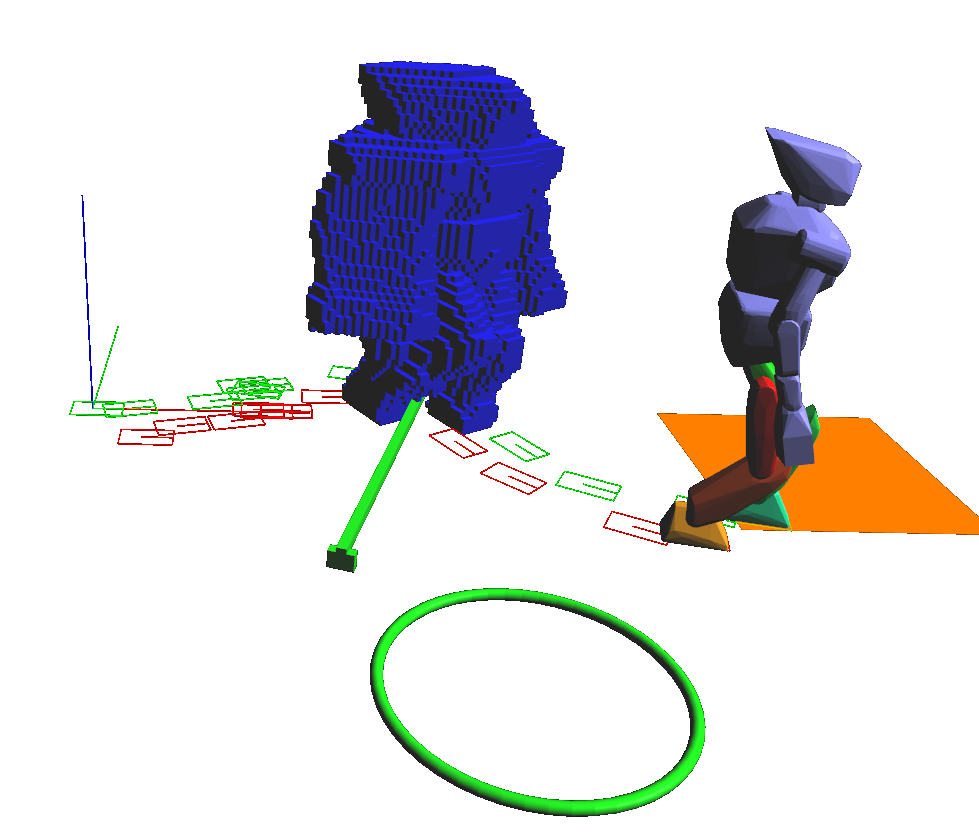
\includegraphics[width=7cm]{./images/SV.png}
    \end{figure}
    Utilisation de PQP avec des volumes balayés.
  \end{center}
\end{frame}

\begin{frame}
  \center Approximation des volumes balayés
  \begin{tiny}
    \begin{figure}
      \subfigure[\tiny{Original - 1.687.596}]{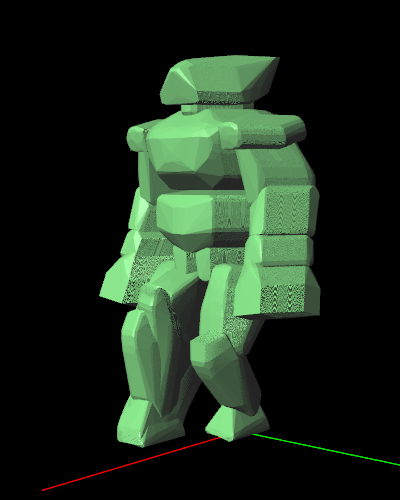
\includegraphics[width=2.5cm]{./images/SV_original.png}}~
      \subfigure[\tiny{5mm - 508.120}]{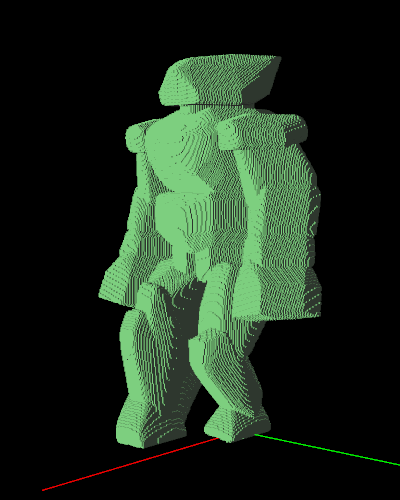
\includegraphics[width=2.5cm]{./images/SV_5mm.png}}~
      \subfigure[\tiny{10mm - 125.772}]{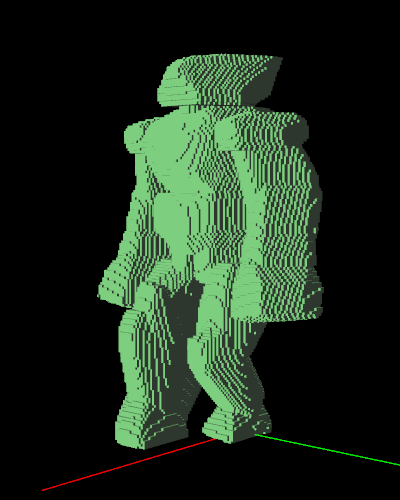
\includegraphics[width=2.5cm]{./images/SV_10mm.png}}
    \end{figure}
    \vspace{-7mm}
    \begin{figure}
      \subfigure[\tiny{25mm - 19.524}]{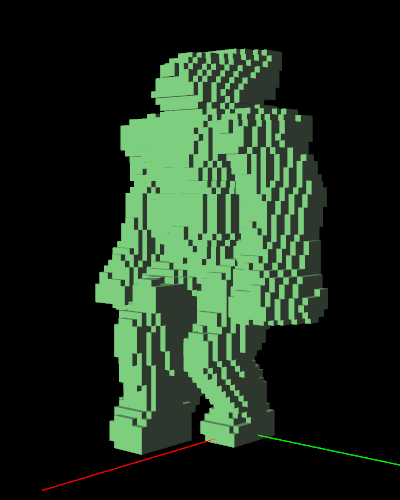
\includegraphics[width=2.5cm]{./images/SV_25mm.png}}~
      \subfigure[\tiny{50mm - 4.596}]{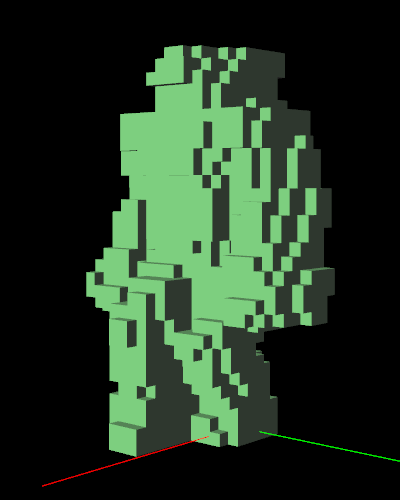
\includegraphics[width=2.5cm]{./images/SV_50mm.png}}~
      \subfigure[\tiny{100mm - 1.144}]{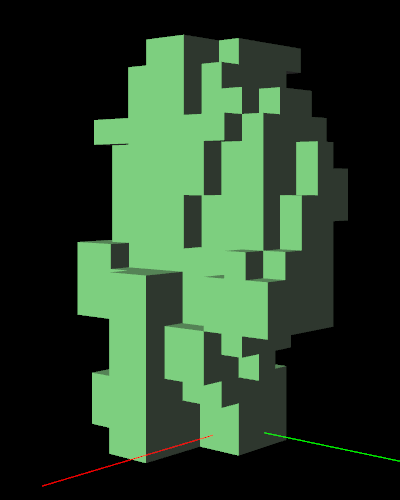
\includegraphics[width=2.5cm]{./images/SV_100mm.png}}
    \end{figure}
  \end{tiny}
\end{frame}

\subsection{Lissage de trajectoire}
\begin{frame}
  \begin{center} 
    Accélération des trajectoires
    \begin{figure}
      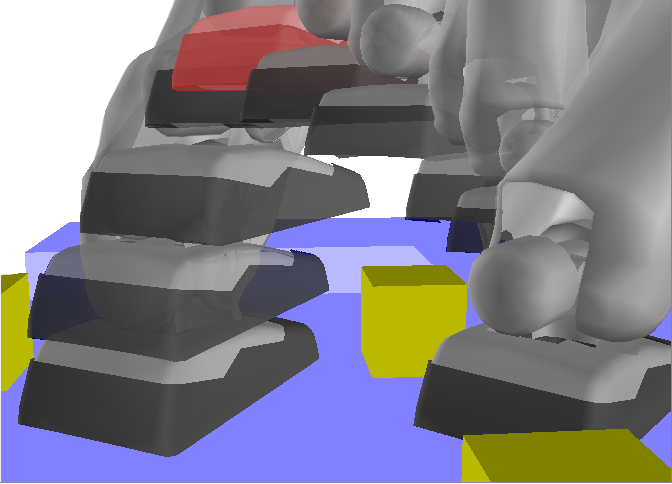
\includegraphics[width=5cm]{./images/smoothing_before.png}~
      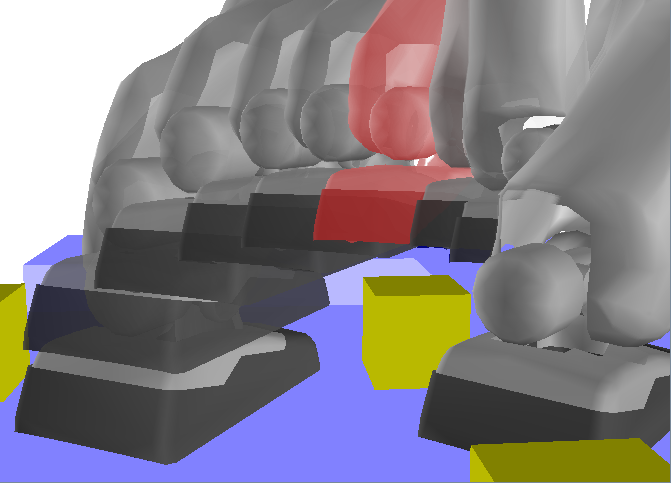
\includegraphics[width=5cm]{./images/smoothing_after.png}
    \end{figure}
    
    Suppression de la phase de double support\\
    Réduction au mieux de la phase de simple support
  \end{center}
\end{frame}

% --------------

\section{Contrôle}
\subsection{Communications - Corba}
\begin{frame}
  \begin{center}
    Organisation de l'informatique embarquée
    \begin{figure}
      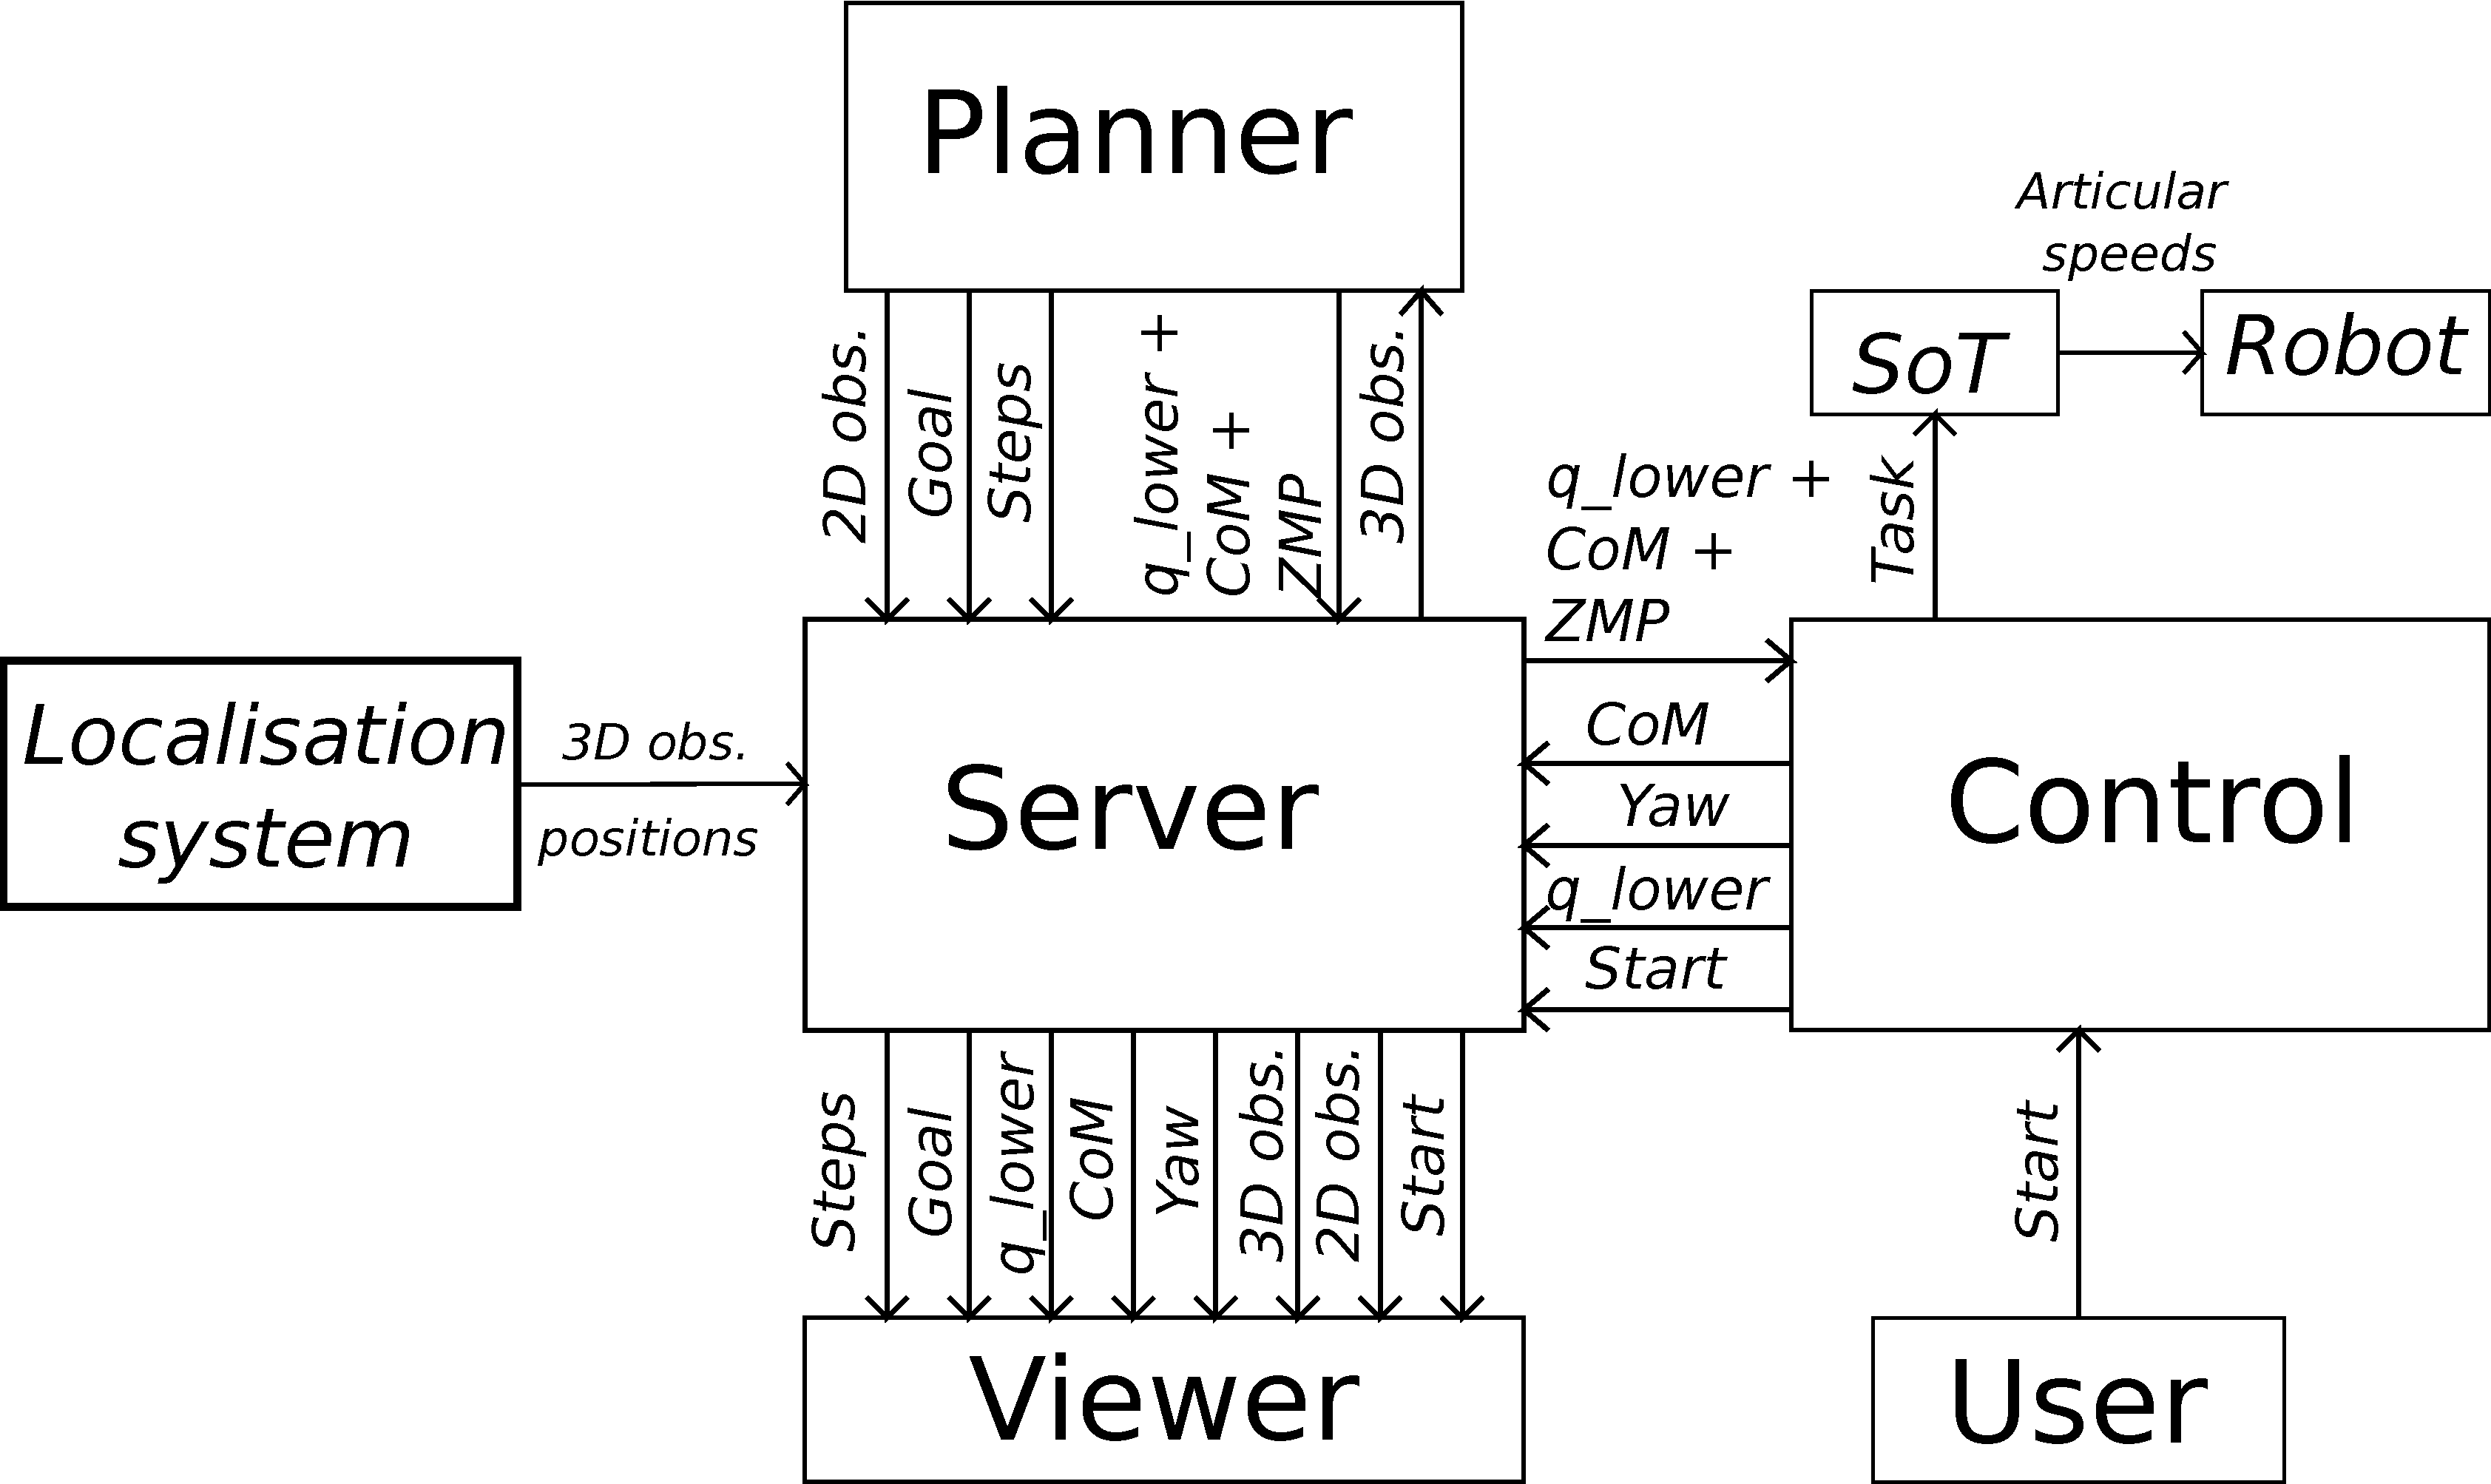
\includegraphics[width=8cm]{./images/corba.png}
    \end{figure}
  \end{center}
\end{frame}

\subsection{Stack of Task - SoT}
\begin{frame}
  \begin{center}
    Gestion des tâches
    \begin{figure}
      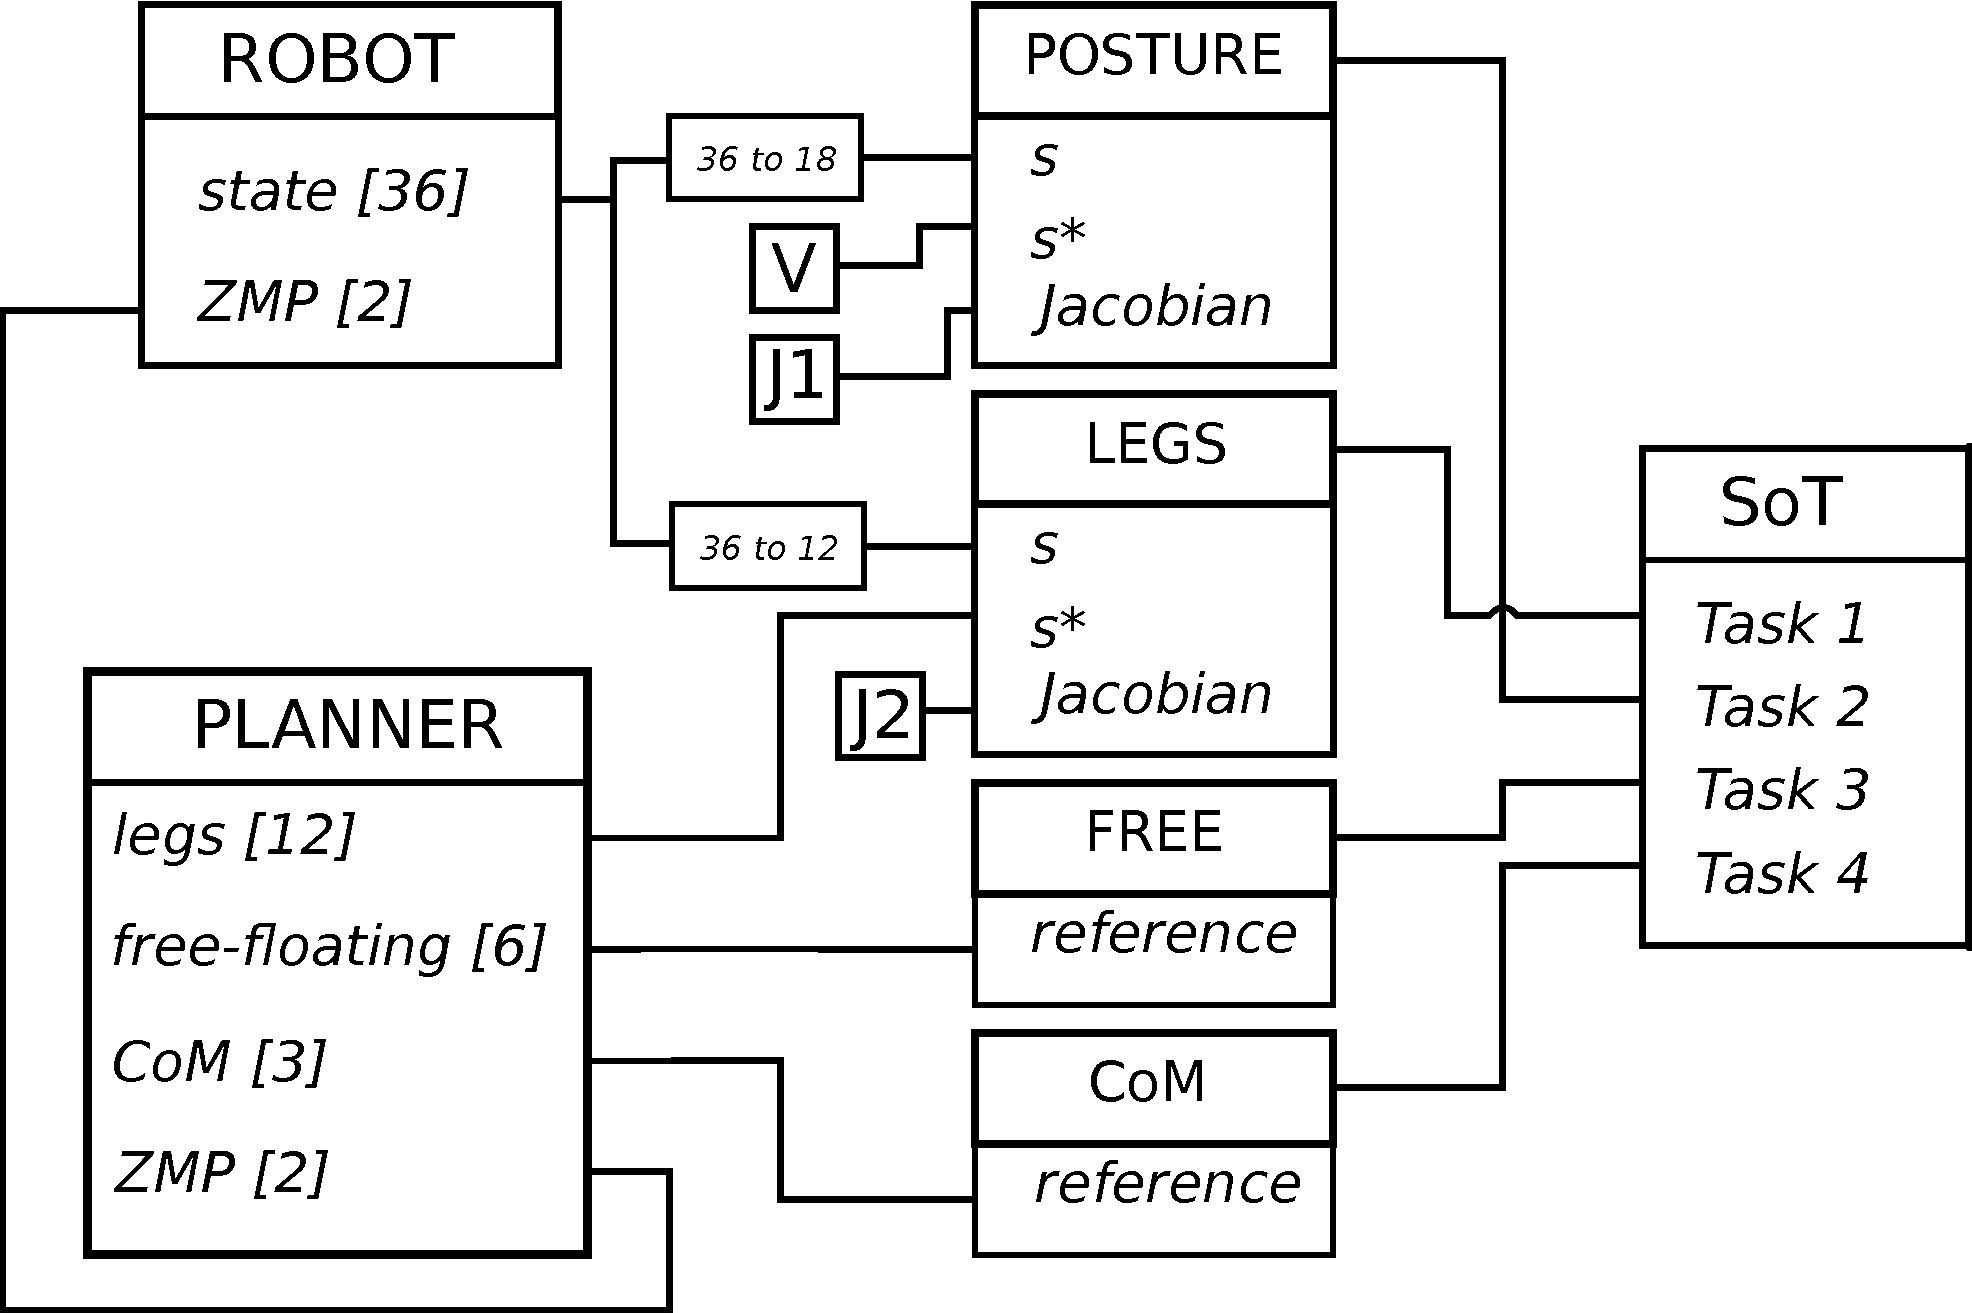
\includegraphics[width=7cm]{./images/SoT.png}
    \end{figure}

    \begin{small}
      \emph{Task Sequencing for High Level Sensor-Based Control}\\
      N. Mansard and F. Chaumette\\
      \textit{IEEE Transactions on Robotics, pages 60–72, 2007.}
  \end{small}
  \end{center}
\end{frame}

% --------------

\section{Expériences}
\subsection{Matériel}
\begin{frame}
  \begin{figure}
    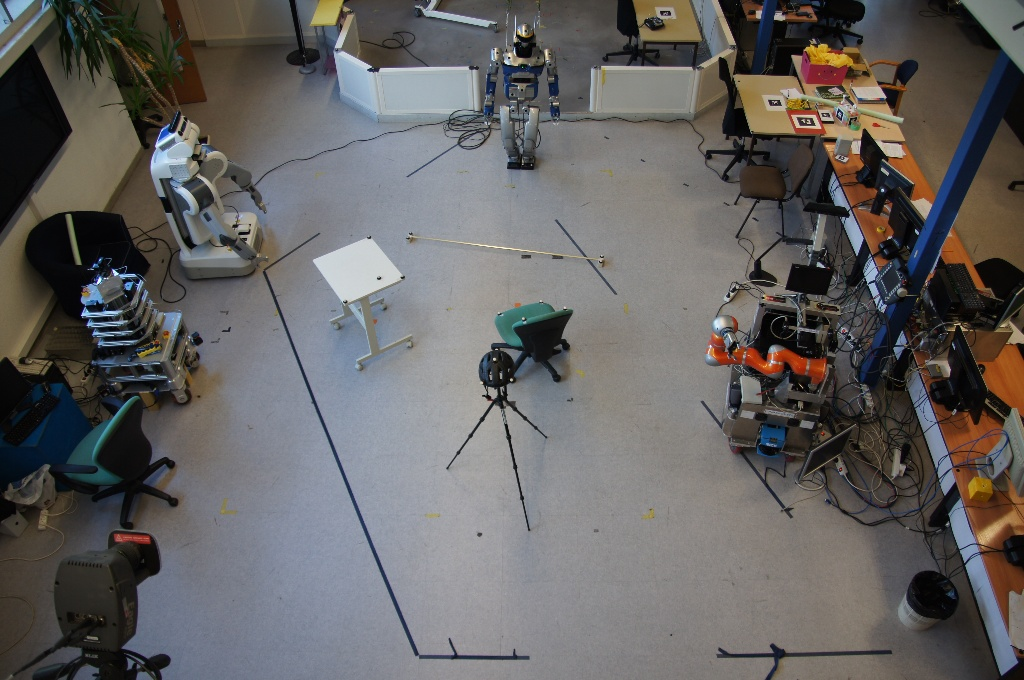
\includegraphics[width=9cm]{./images/grande_salle.jpg}\\
    Grande salle d'expérience robotique du LAAS.
  \end{figure}
\end{frame}

\subsection*{Motion capture}
\begin{frame}
  \center Détection des différents objets avec la \textit{motion capture}.\\
   \begin{figure}
    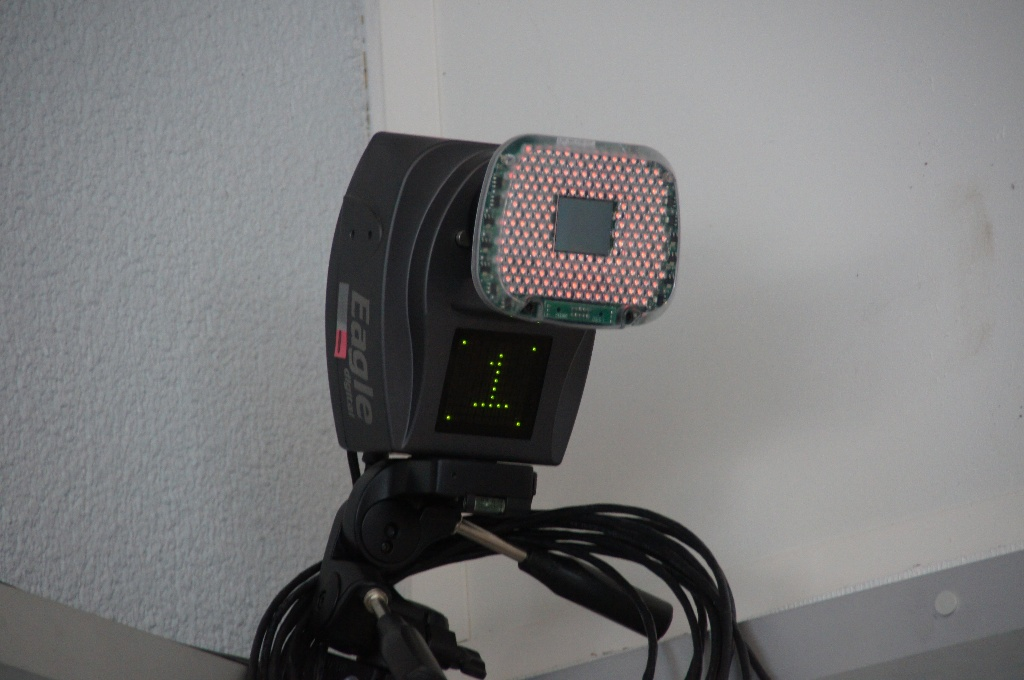
\includegraphics[width=4.5cm]{./images/IR.jpg}~
    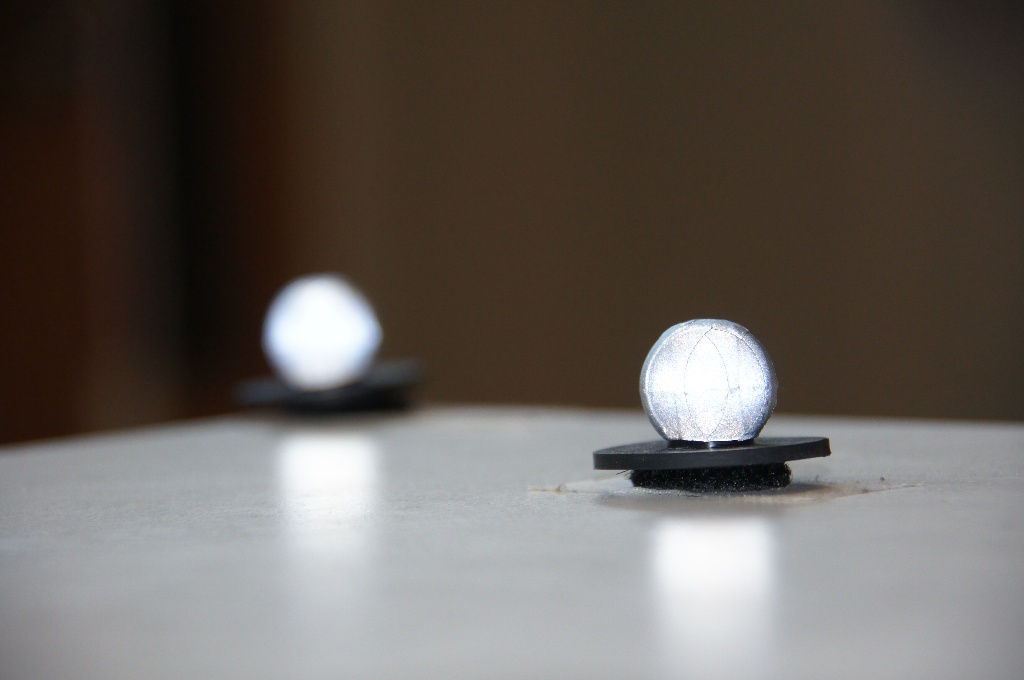
\includegraphics[width=4.5cm]{./images/marker_flash.jpg}
  \end{figure}
  \vspace{-5mm}
  \begin{figure}
    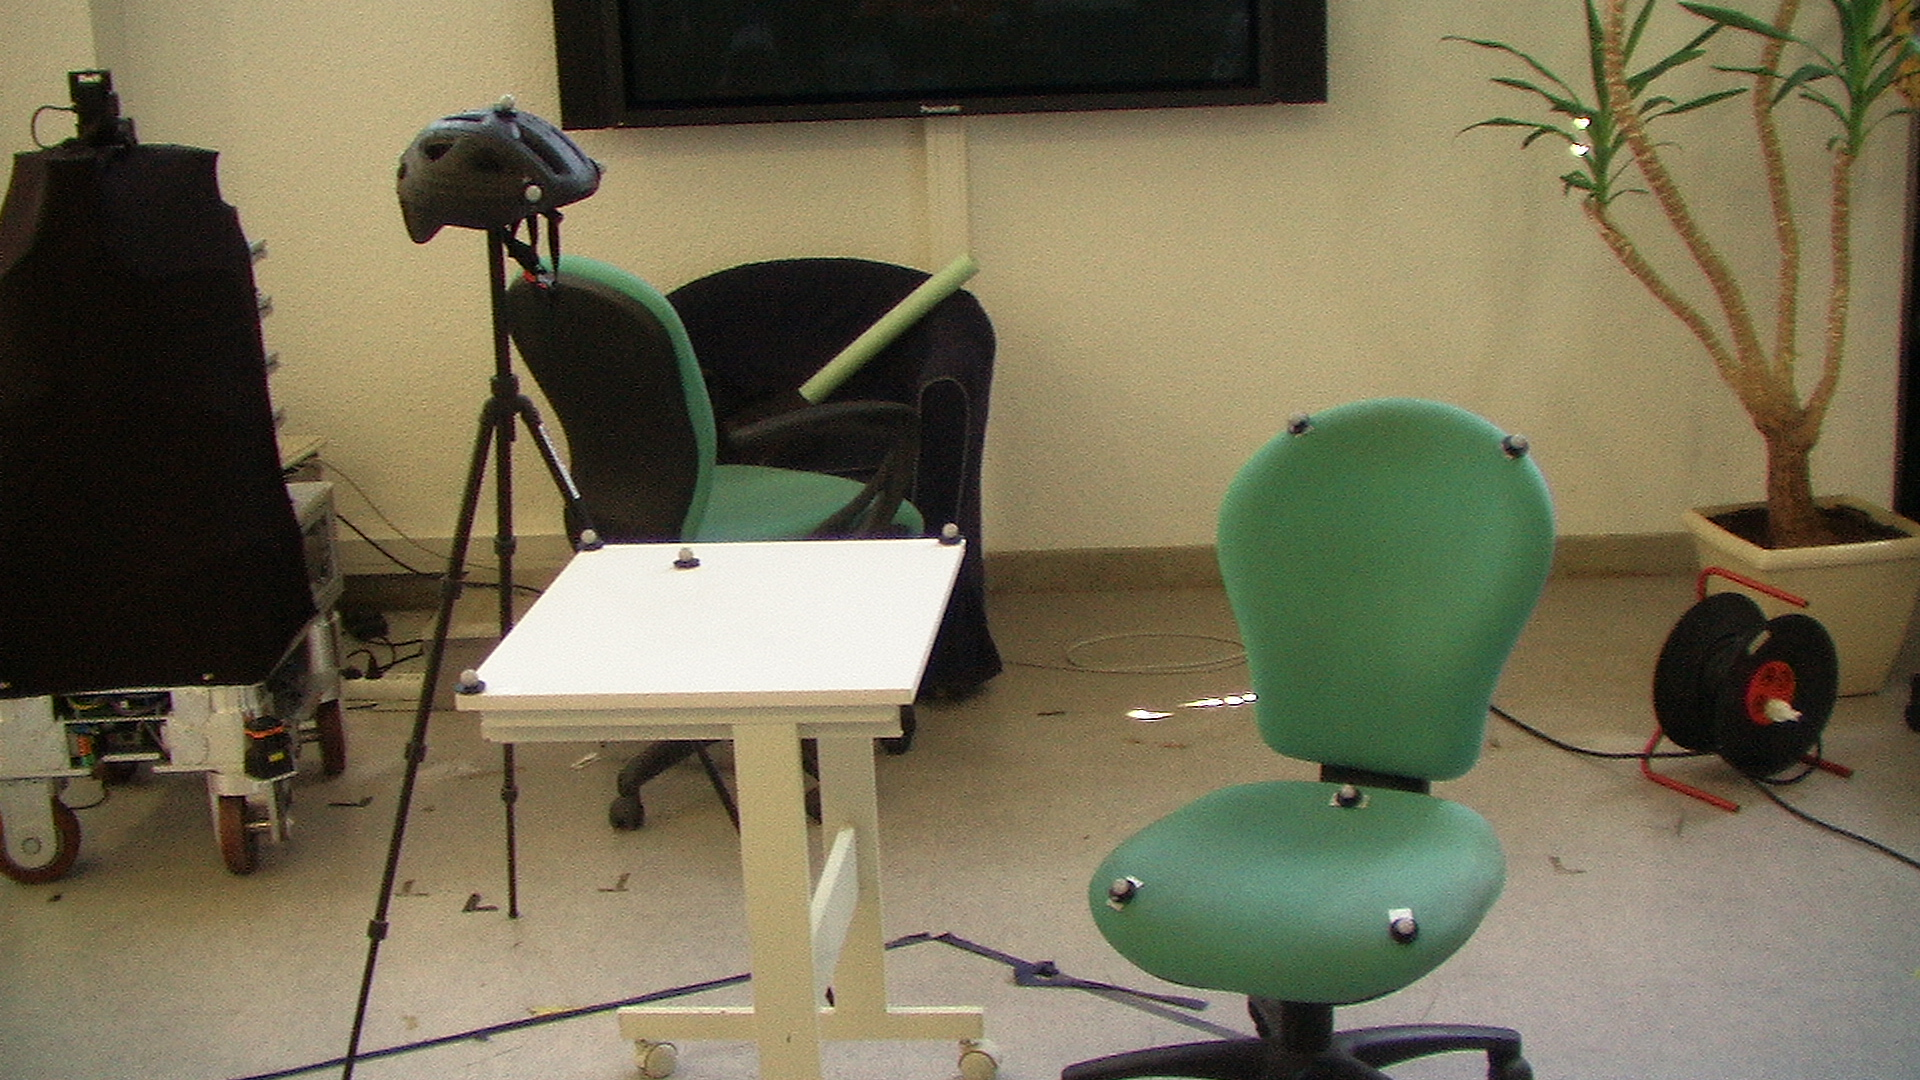
\includegraphics[width=5cm]{./images/mocap_real.jpg}~
    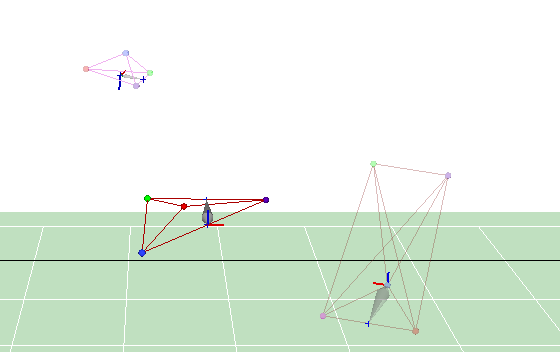
\includegraphics[width=5cm]{./images/mocap.png}
  \end{figure}
\end{frame}

\subsection{Résultats}
\begin{frame}
  \begin{figure}
    \movie{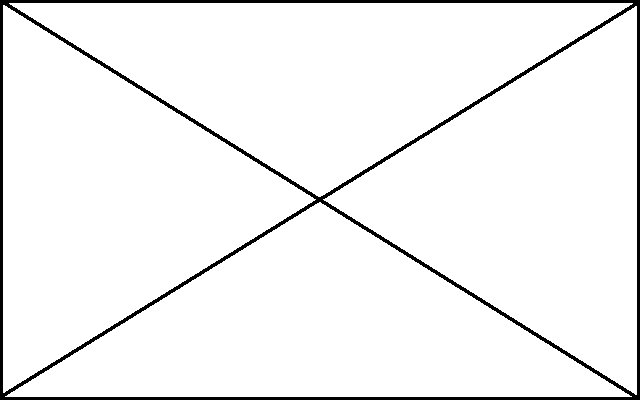
\includegraphics[width=9cm]{./images/vide.jpg}}{./videos/humanoids-17-08-11-a.avi}\\
    Vidéo soumise à Humanoids'11
   \end{figure}
 \end{frame}

\begin{frame}
  \begin{itemize}
  \item  Performances :
    \begin{itemize}
    \item Vitesse de planification
    \item Enjambement d'obstacles
    \item Replanification
    \end{itemize}
    \vspace{3mm}
  \item Points restants à améliorer :
    \begin{itemize}
    \item Vitesse de marche du robot
    \item Précision sur la position du pied
    \item Rendre le robot autonome
    \end{itemize}
  \end{itemize}
\end{frame}

% --------------

\section{Conclusion}
\subsection*{Publications}
\begin{frame}
  \begin{itemize}
    \item Transactions on Robotics :\\
N. Perrin, O. Stasse, \textbf{L. Baudouin}, F. Lamiraux, and E. Yoshida. \emph{Fast Humanoid Robot Collision-Free Footstep Planning Using Swept Volume Approximations}. \textit{IEEE Transactions on Robotics}, 2011. conditionnally accepted.

    \item Humanoids :\\
\textbf{L. Baudouin}, N. Perrin, O. Stasse, T. Moulard, E. Yoshida, and F. Lamiraux. \emph{Real-time Replanning Using 3D Environment for Humanoid Robot}.
In \textit{IEEE Int. Conf. on Humanoid Robotics (Humanoids’11)}, 2011.


    \item Robotics Society of Japan :\\
\textbf{L. Baudouin}, N. Perrin, O. Stasse, T. Moulard, E. Yoshida, and F. Lamiraux. \emph{Real-time Replanning Using 3D Environment for Humanoid Robot}.
In \textit{RSJ11}, 2011.
      
  \end{itemize}
\end{frame}

\subsection*{Conclusion Générale}
\begin{frame}
  \begin{itemize}
  \item Travaux de recherche
    \begin{itemize}
    \item Intérêts
    \item Difficultés
    \item Publications
   \end{itemize}
  \item Programmation
    \begin{itemize}
    \item Packaging
    \item Langages
    \end{itemize}
  \item Poursuite du projet
    \begin{itemize}
    \item Applications
    \item Limites
    \end{itemize}
  \end{itemize}
\end{frame}

\subsection*{Discussion}
\begin{frame}
  \begin{center}
    \textit{Merci pour votre attention.}\\
    \huge{Avez-vous des questions ?}
  \end{center}
\end{frame}

%% -------------

\end{document}  
